
\chapter{Hardware Architecture}

\section{Overview}

This DLX is a 32-bit RISC processor with a five-stage pipeline. The external interface is made mainly for memories connection (IRAM, DRAM and a DRAM for the Register File), and for the Clock and Reset signals. Inside we find the following blocks:

\begin{itemize}
    \item Control Unit: it receives the fetched instruction from the IR register and starts to output the correct control signals towards all the pipeline stages. Moreover, it receives status signals from all other units about their working status like the comparator result (for branch decision), the status about possible hazards in the pipeline, Register File's Push \& Pop operations under execution, and all the memories readiness. It's in charge of controling the entire pipeline and stop it in case of hazards or other situations that requires a stall.
    \item Decode Unit: part of the decode stage, it is in charge of keeping the status about all registers under use (for further hazard controls), computation of the new Program Counter (given a Jump or not), data comparison (for branches) and, the most important thing, the operation decode with the dispatch of all the operands towards the right ports of the DataPath.
    \item DataPath: the computational core of the processor. Made of 4 pipeline stages (Instruction Decode, Execution, Memory, Write Back) contains all the units capable of doing computation. In particular, we have the Register File (that manages all the registers of the core), the Arithmetic Logic Unit, the Load-Store Unit for data memory management, and other units useful for the correct operation of everything.
    \item IR and PC: two registers the compose the Instruction Fetch stage of the pipeline, they are in charge of keeping in memory the current instruction under execution and the address for the next instruction to execute, respectively. 
\end{itemize}


\begin{figure}[ht]
    \centering
    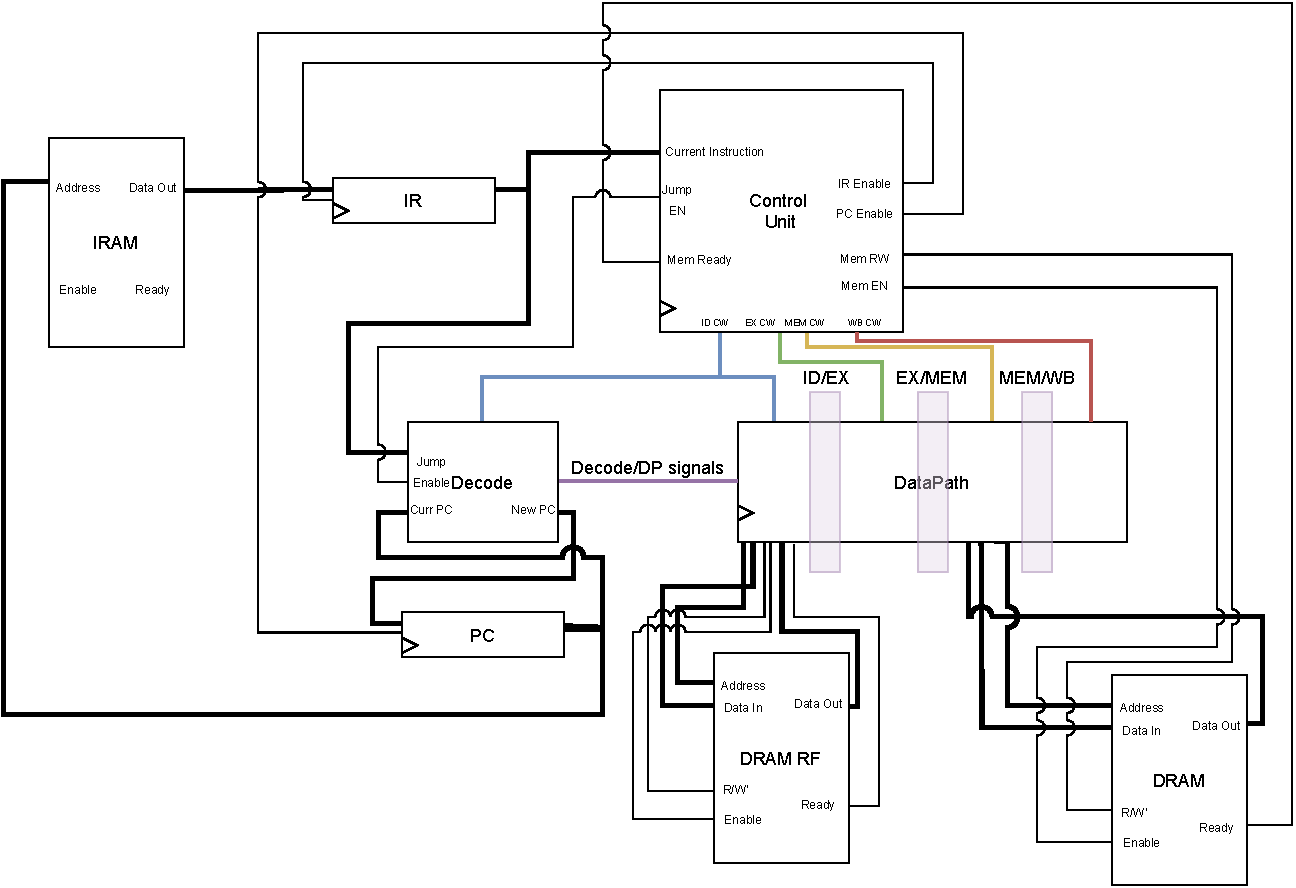
\includegraphics[width=1\textwidth]{chapters/2_dlx/images/DLX.pdf}
    \caption{Schematic of the DLX}
    \label{DLX}
\end{figure} 
\newpage
\section{Pipeline Stages}
\section{Control Unit}
\section{Memory Interface}

The DLX processor has a Harvard architecture, with two 32-bit data bus carrying instructions and data respectively. Only load and store instructions can access data from Data Memory. The Data are stored in memory in a Big-Endian format.\\

The third RAM required, the one for the register file, is not under the direct access of the User. It's managed as a Stack memory by the Register File for automatic sub routines management and it has a dedicated interface. It can be merged with the Data Memory with an external logic.\\


All the subsequent paragraph are referred in the same way to all the three memory types.

\subsection{Signals and Timing}
The signals in the DLX processor bus interface can be grouped into tree categories:
\begin{itemize}
    \item Address class signals
    \item Memory Request signals
    \item Data class signals
\end{itemize}

The \emph{Address class signals} are:
\begin{itemize}
    \item A{[31:0]}
    \item DATA\_SIZE{[1:0]} \emph{or MAS{[1:0]}}
\end{itemize}

The \emph{Memory Request signals} are:
\begin{itemize}
    \item Enable
    \item $R\overline{W}$
    \item Ready
\end{itemize}

Moreover, all the memories connected must agree on a certain protocol both for writing and reading operations. The most important thing to take under consideration is the \emph{Ready} signal: it must be high only when the operation is really completed. For example after a data read, the \emph{Ready} stays at 1 only when the data is valid. If meanwhile the address changes, the \emph{Ready} signal must go off.

\begin{tikztimingtable}[%
    timing/dslope=0.2,
    timing/.style={x=8ex,y=2ex},
    x=8ex,
    timing/rowdist=3ex,
    timing/name/.style={font=\sffamily\scriptsize}
]
    \busref{CLK}                & 16{c} \\
    \busref[31:0]{Address}      & 2x 1D{$A_1$} 2D{$A_2$} 1X 1D{$A_4$} UX \\
    \busref[1:0]{MAS}           & 2x 1D{WORD 00} 2D{HALF 01} X 1D{BYTE 10} 2X\\
    \busref{Enable}             & 1L 2H HL HL L\\
    \busref{$RnW$}              & 1L 2H 2H LH L\\
    Ready                       & ll lh lh hh ll lh LL\\
    \busref[31:0]{Data In}      & 2x 2x 1X 1X 1X 1D{$D_1$} XX \\
    \busref[31:0]{DATA Out}      & 2x x1d{$D_1$} x3d{$D_2$} 4X  \\
    \extracode
    \begin{pgfonlayer}{background}
    \begin{scope}[semitransparent ,semithick]
    \vertlines[darkgray,dotted]{0.5,1.5 ,...,8.0}
    \end{scope}
    \end{pgfonlayer}
\end{tikztimingtable}


If the memory in use can't accomplish to this timing, an external \emph{Memory Control Unit} must be placed between the CPU and the Memory.

\subsection{Memory Addressing}
A[31:0] is the 32-bit address bus that specifies the address for the transfer. All addresses are byte addresses, so a burst of word accesses results in the address bus incrementing by four for each cycle.\\

The address bus provides 4GB of linear addressing space, and this can be used externally in different manners like in a SoC with memory mapped peripherals that shares the same address space.\\

When a word access is signaled the memory system ignores the bottom two bits, A[1:0], and when a halfword access is signaled the memory system ignores the bottom bit, A[0]. Howewer, the core already masks the two LSBs when needed.

\subsection{Memory Data Size: the MAS[1:0] signal}

The \emph{MAS[1:0]} bus encodes the size of the transfer. The DLX processor can transfer word, halfword, and byte quantities and the processor indicates the size of the transfer through this signal.\\

When a halfword or byte read is performed, a 32-bit memory system can return the complete 32-bit word, and the processor extracts the valid halfword or byte field from it. For 8 and 16 bit memories, the data must be placed on the right byte lanes in the data bus.

\section{Instruction Set}